To verify the behavior of the solubility limitation model in the Mixed Cell
model, for example, one hundred multi-component simulations were conducted,
each with a different reference solubility limit.
For an arbitrary isotope, the expected solubility
limitation behavior is captured and compared favorably to the Clay \gls{GDSM}
solubility limitation sensitivity results.

The results in Figure \ref{fig:SolSumFactor}, from the detailed parametric
analysis in \cite{huff_key_2012}, showed that for solubility limits below a
certain threshold, the dose releases were directly proportional to the
solubility limit, indicating that the radionuclide concentration saturated the
groundwater up to the solubility limit near the waste form.  For solubility
limits above the threshold, however, further increase to the limit had no
effect on the peak dose. This demonstrates the situation in which the
solubility limit is so high that even complete dissolution of the waste
inventory into the pore water is insufficient to reach the solubility limit.


\begin{figure}[ht]
\begin{center}
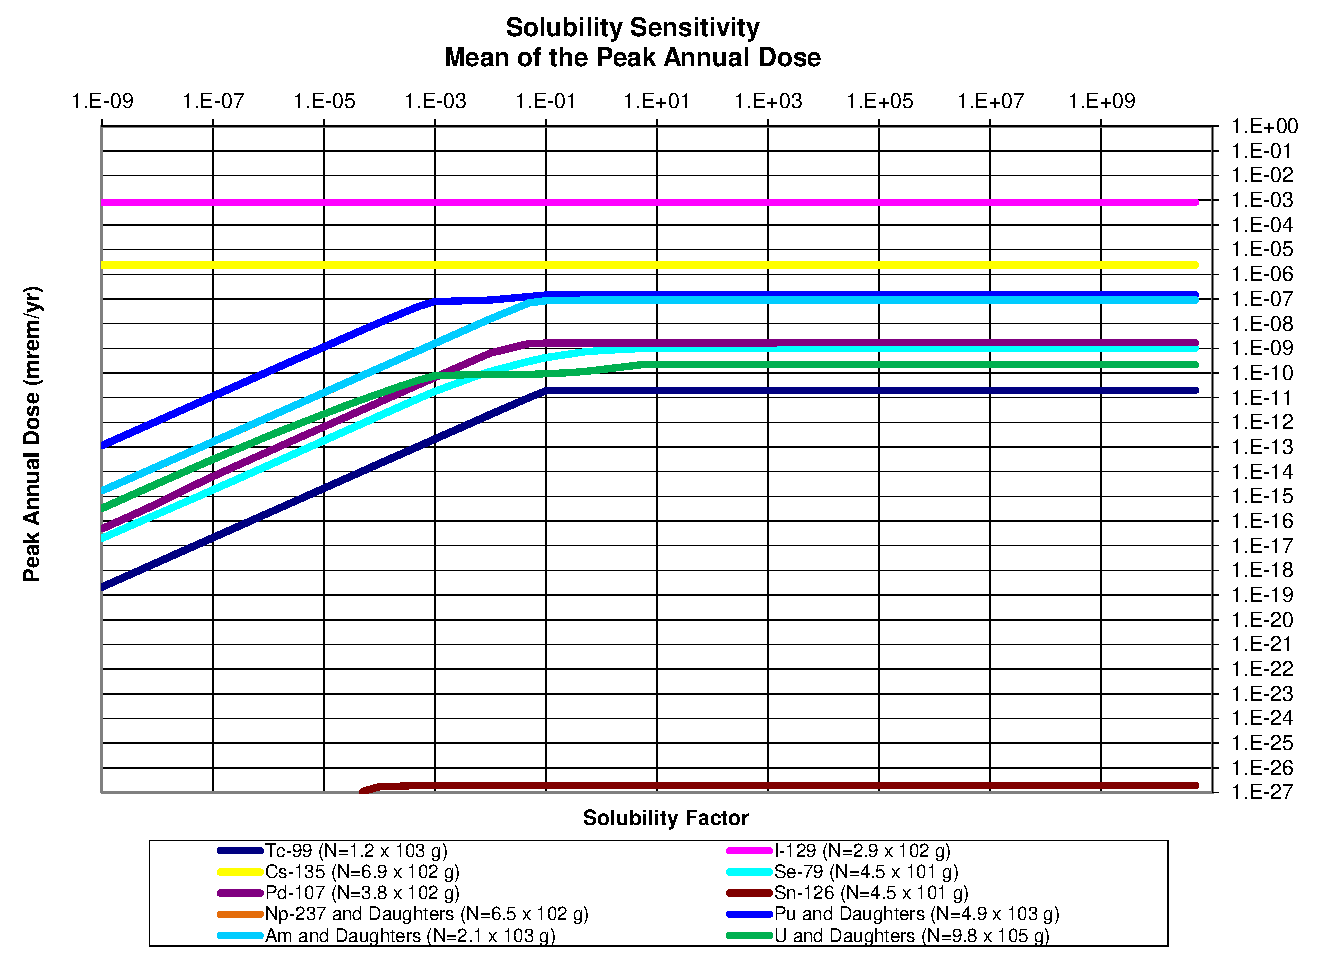
\includegraphics[width=0.7\linewidth]{./results/images/Solubility_Summary_SolFactor.eps}
\caption[Solubility factor sensitivity in the Clay GDSM model]{Solubility
        factor sensitivity in the DOE Clay GDSM, reproduced from 
        \cite{huff_key_2012}. The peak annual dose due to an inventory, $N$, of each
isotope. This result was achieved with a parametric analysis using a detailed
        model of a generic clay repository.}
\label{fig:SolSumFactor}
\end{center}
\end{figure}

\begin{figure}[ht]
\begin{center}
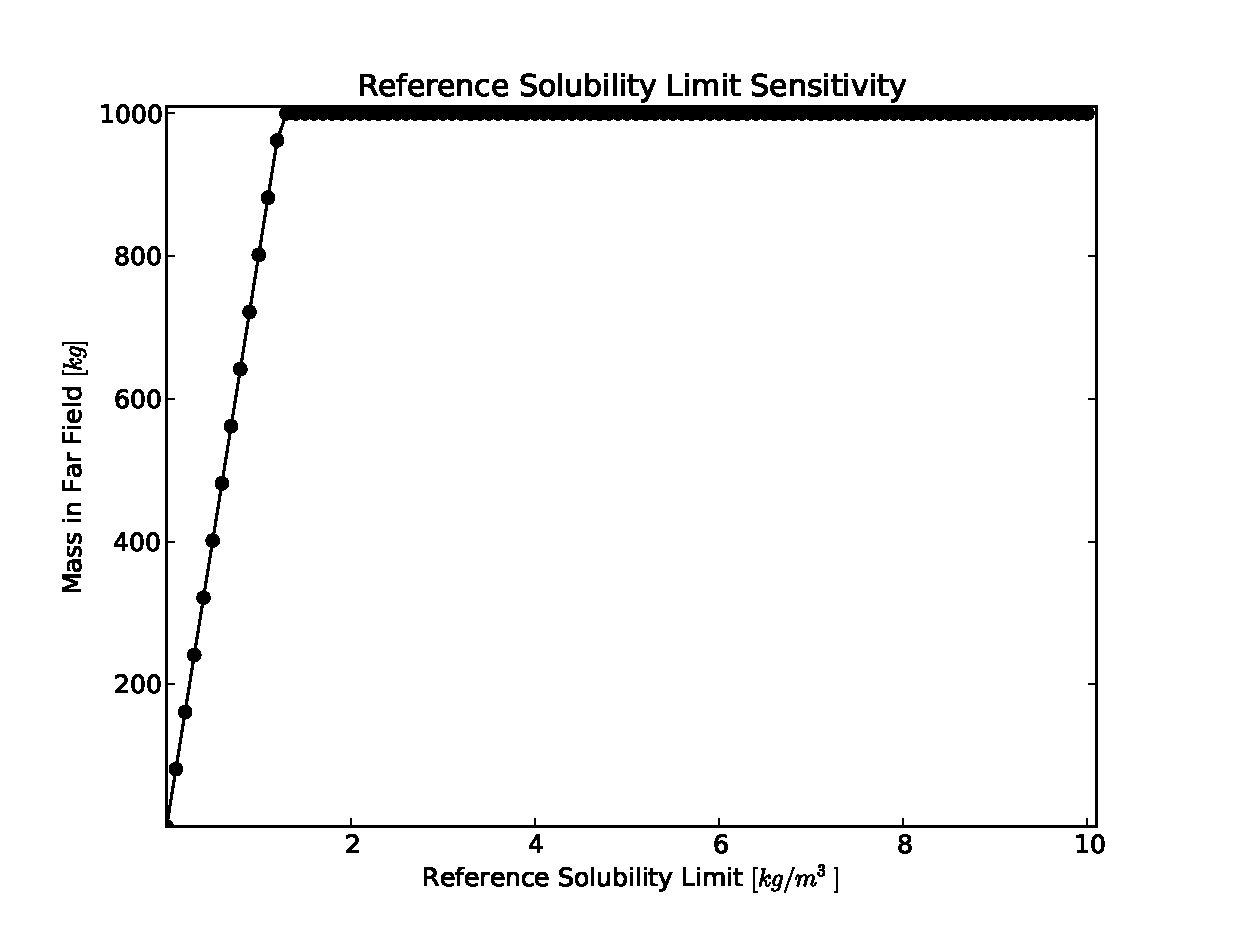
\includegraphics[width=0.7\linewidth]{./results/images/sol.eps}
\caption[Solubility Sensitivity in the Mixed Cell Model]{Sensitivity demonstration of solubility limitation in \Cyder for an arbitrary isotope assigned a variable solubility limit.}
\label{fig:sol_result}
\end{center}
\end{figure}


In the corresponding parametric analysis of \Cyder performance, it was shown that the
solubility sensitivity behavior closely matched that of the \gls{GDSM}
sensitivity behaviors. Specifically, in Figure \ref{fig:sol_result}, a marked 
transition to the solubility-limited regime
is seen where the solubility limit exceeds the point at which it limits
movement. For increased solubility limits, release remains constant, as
expected.

In both \Cyder and the more detailed Clay \gls{GDSM}, for solubility constants
lower than the saturation threshold, the transport regime is solubility
limited and the relationship between peak annual dose and solubility limit is
strong.  Above the threshold, the transport regime is inventory limited
instead.

%\begin{figure}[ht]
%\begin{center}
%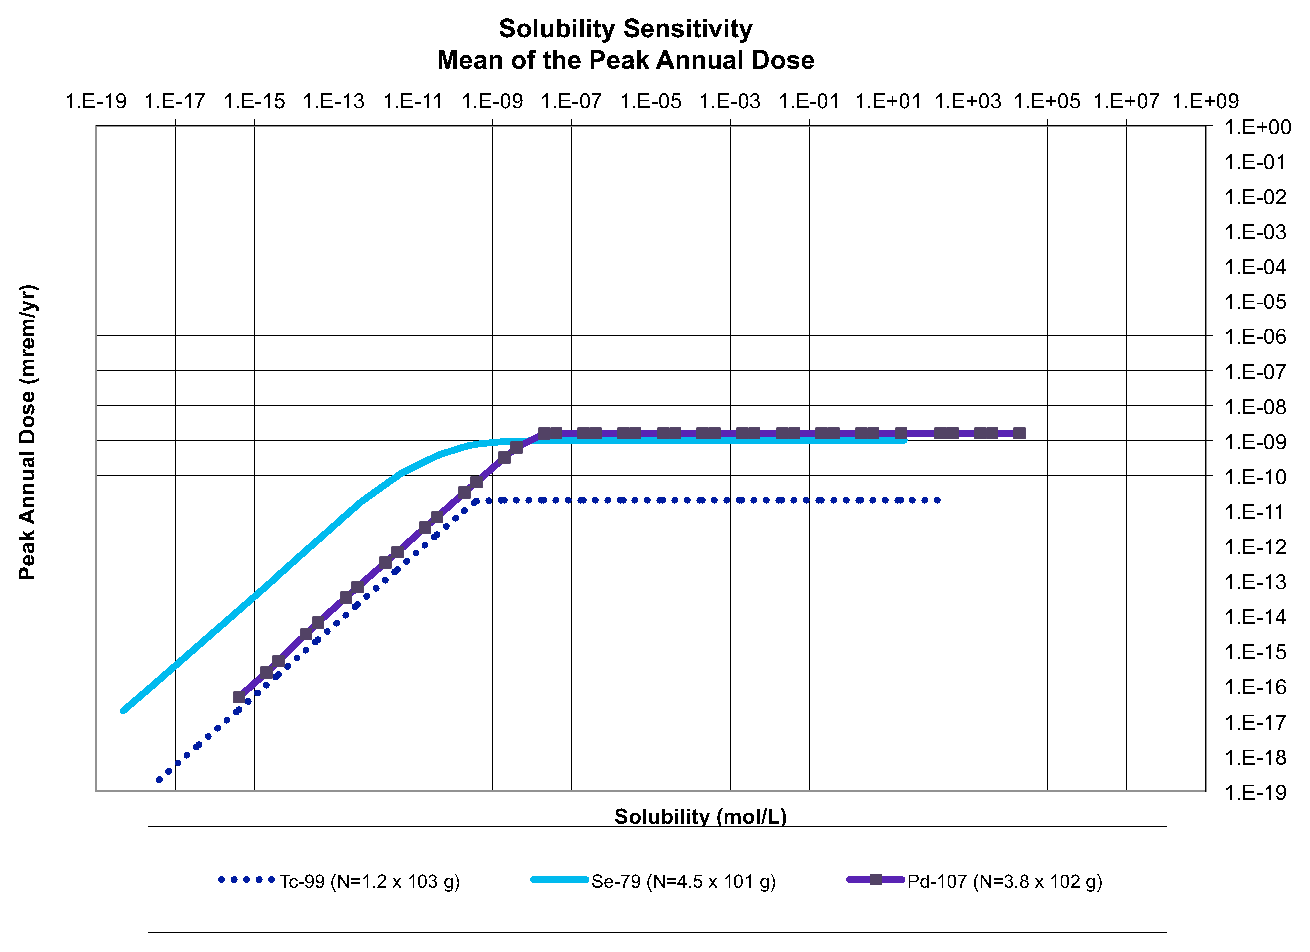
\includegraphics[width=0.7\linewidth]{./results/images/Solubility_Summary_Sol.eps}
%\caption[Solubility limit sensitivity in GDSM Clay model]{Solubility limit sensitivity. The peak annual dose due to an inventory,
%$N$, of each isotope.}
%\label{fig:SolSum}
%\end{center}
%\end{figure}

